\documentclass[UTF8]{ctexart}
\usepackage{amsmath}
\usepackage{xfrac}


\title{你好,world!}
\author{Liam}
\date{\today}

\usepackage{setspace}
\onehalfspacing
\addtolength{\parskip}{.4em}

\usepackage{geometry}
\geometry{papersize={20cm,15cm}}
\geometry{left=1cm,right=2cm,top=3cm,bottom=4cm}

\usepackage{fancyhdr}
\pagestyle{fancy}
\lhead{\author}
\chead{\date}
\rhead{152xxxxxxxx}
\lfoot{}
\cfoot{\thepage}
\rfoot{}
\renewcommand{\headrulewidth}{0.4pt}
\renewcommand{\headwidth}{\textwidth}
\renewcommand{\footrulewidth}{0pt}

\begin{document}

\maketitle
\tableofcontents


\section{启动 TeXworks}
启动 TeXworks 很简单,你可以在 Windows 启动对话框中输入 texworks 按回车。

\section{实现中英文混排}
在 TeXworks 编辑框中输入以下内容,以 UTF-8 编码保存,使用 XeLaTeX 编译:
documentclass[UTF8]{ctexart}

\section{组织你的文章}
%\documentclass[UTF8]{ctexart}
%\title{你好,world!}
%\author{Liam}
%\date{\today}
%\begin{document}
%\maketitle
%你好,world!
%\end{document}

\subsection{作者、标题、日期}

\section{数学模式}
\subsection{ 上下标}
Einstein 's $E=mc^2$.

\[ E=mc^2. \]

\begin{equation}
E=mc^2.
\end{equation}

\subsection{ 根式与分式}

$\sqrt{x}$, $\frac{1}{2}$.

\[ \sqrt{x}, \]

\[ \frac{1}{2}. \]

\subsection{ 运算符}

\[ \pm\; \times \; \div\; \cdot\; \cap\; \cup\;
\geq\; \leq\; \neq\; \approx \; \equiv \]

$ \sum_{i=1}^n i\quad \prod_{i=1}^n $

$ \sum\limits  _{i=1}^n i
\quad \prod\limits _{i=1}^n $


\[ \lim_{x\to0}x^2 \quad \int_a^b x^2 dx \]
\[ \lim\nolimits _{x\to0}x^2\quad \int\nolimits_a^b x^2 dx \]

\[ \lim\nolimits _{x\to0}x^2                              \int\nolimits_a^b x^2 dx \]

\paragraph{积分}

\[ \iint\quad \iiint\quad \iiiint\quad \idotsint \]

\subsection{ 定界符(括号等)}
\[ ( ) \]


\[ \{ \} \]

\[ \lvert \rvert \]

\[ \lVert \rVert \]

\[ \Biggl(\biggl(\Bigl(\bigl((x)\bigr)\Bigr)\biggr)\Biggr) \]
\[ \Biggl[\biggl[\Bigl[\bigl[[x]\bigr]\Bigr]\biggr]\Biggr] \]
\[ \Biggl \{\biggl \{\Bigl \{\bigl \{\{x\}\bigr \}\Bigr \}\biggr \}\Biggr\} \]
\[ \Biggl\langle\biggl\langle\Bigl\langle\bigl\langle\langle x
\rangle\bigr\rangle\Bigr\rangle\biggr\rangle\Biggr\rangle \]
\[ \Biggl\lvert\biggl\lvert\Bigl\lvert\bigl\lvert\lvert x
\rvert\bigr\rvert\Bigr\rvert\biggr\rvert\Biggr\rvert \]
\[ \Biggl\lVert\biggl\lVert\Bigl\lVert\bigl\lVert\lVert x
\rVert\bigr\rVert\Bigr\rVert\biggr\rVert\Biggr\rVert \]

\subsection{省略号}
\[ x_1,x_2,\dots ,x_n\quad 1,2,\cdots ,n\quad
\vdots\quad \ddots \]

\subsection{矩阵}

\[ \begin{pmatrix}
 a&b\\
 c&d 
 \end{pmatrix} \quad
\begin{bmatrix} a&b\\c&d \end{bmatrix} \quad
\begin{Bmatrix} a&b\\c&d \end{Bmatrix} \quad
\begin{vmatrix} a&b\\c&d \end{vmatrix} \quad
\begin{Vmatrix} a&b\\c&d \end{Vmatrix} 
\]

\paragraph{small matrix}
Marry has a little matrix $ ( \begin{smallmatrix} a&b\\c&d \end{smallmatrix} ) $.

\subsection{多行公式}
\subsubsection{长公式}
\paragraph{长公式}
\subparagraph{不对齐}
\begin{multline}
x = a+b+c+{} \\
d+e+f+g
\end{multline}

\subparagraph{对齐}
\[
\begin{aligned}
x ={}& a+b+c+{} \\
&d+e+f+g
\end{aligned}
\]
\subsubsection{公式组}
无需对齐的公式组可以使用 gather 环境,需要对齐的公式组可以使用 align 环境。他们都带有编号,如果不需要编号可以使用带星花的版本。
\begin{gather}
a = b+c+d \\
x = y+z
\end{gather}
\begin{align}
a &= b+c+d \\
x &= y+z
\end{align}

\[ y= \begin{cases}

-x,\quad & x\leq 0 \\
x,\quad & x\geq 0

\end{cases} \]

\subsection{ 插入图片和表格}
\subsubsection{图片}

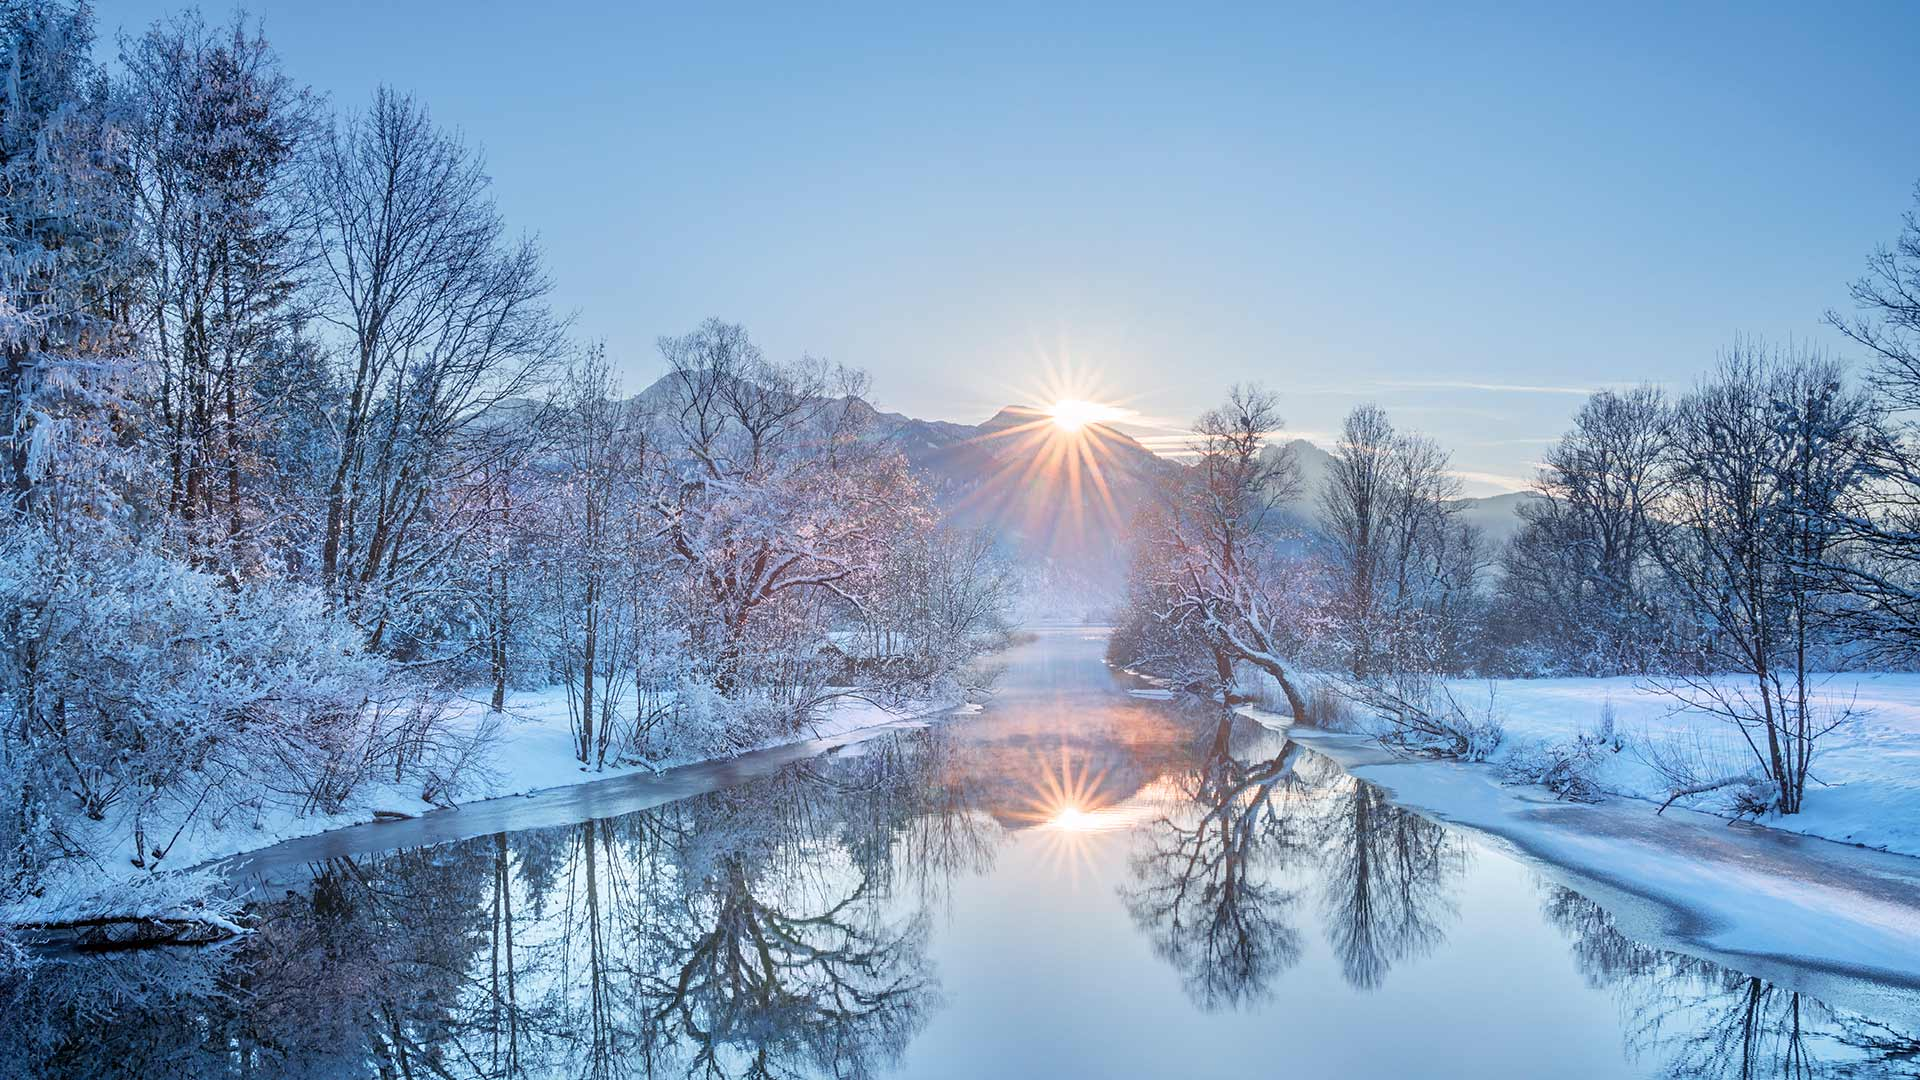
\includegraphics[width = .9\textwidth]{a.jpg}

\subsubsection{表格}

\begin{tabular}{|l|c|r|}
 \hline
操作系统& 发行版& 编辑器\\
 \hline
Windows & MikTeX & TexMakerX \\
 \hline
Unix/Linux & teTeX & Kile \\
 \hline
Mac OS & MacTeX & TeXShop \\
 \hline
通用& TeX Live & TeXworks \\
 \hline
\end{tabular}

\subsubsection{浮动体}

\begin{figure}[htbp]
\centering
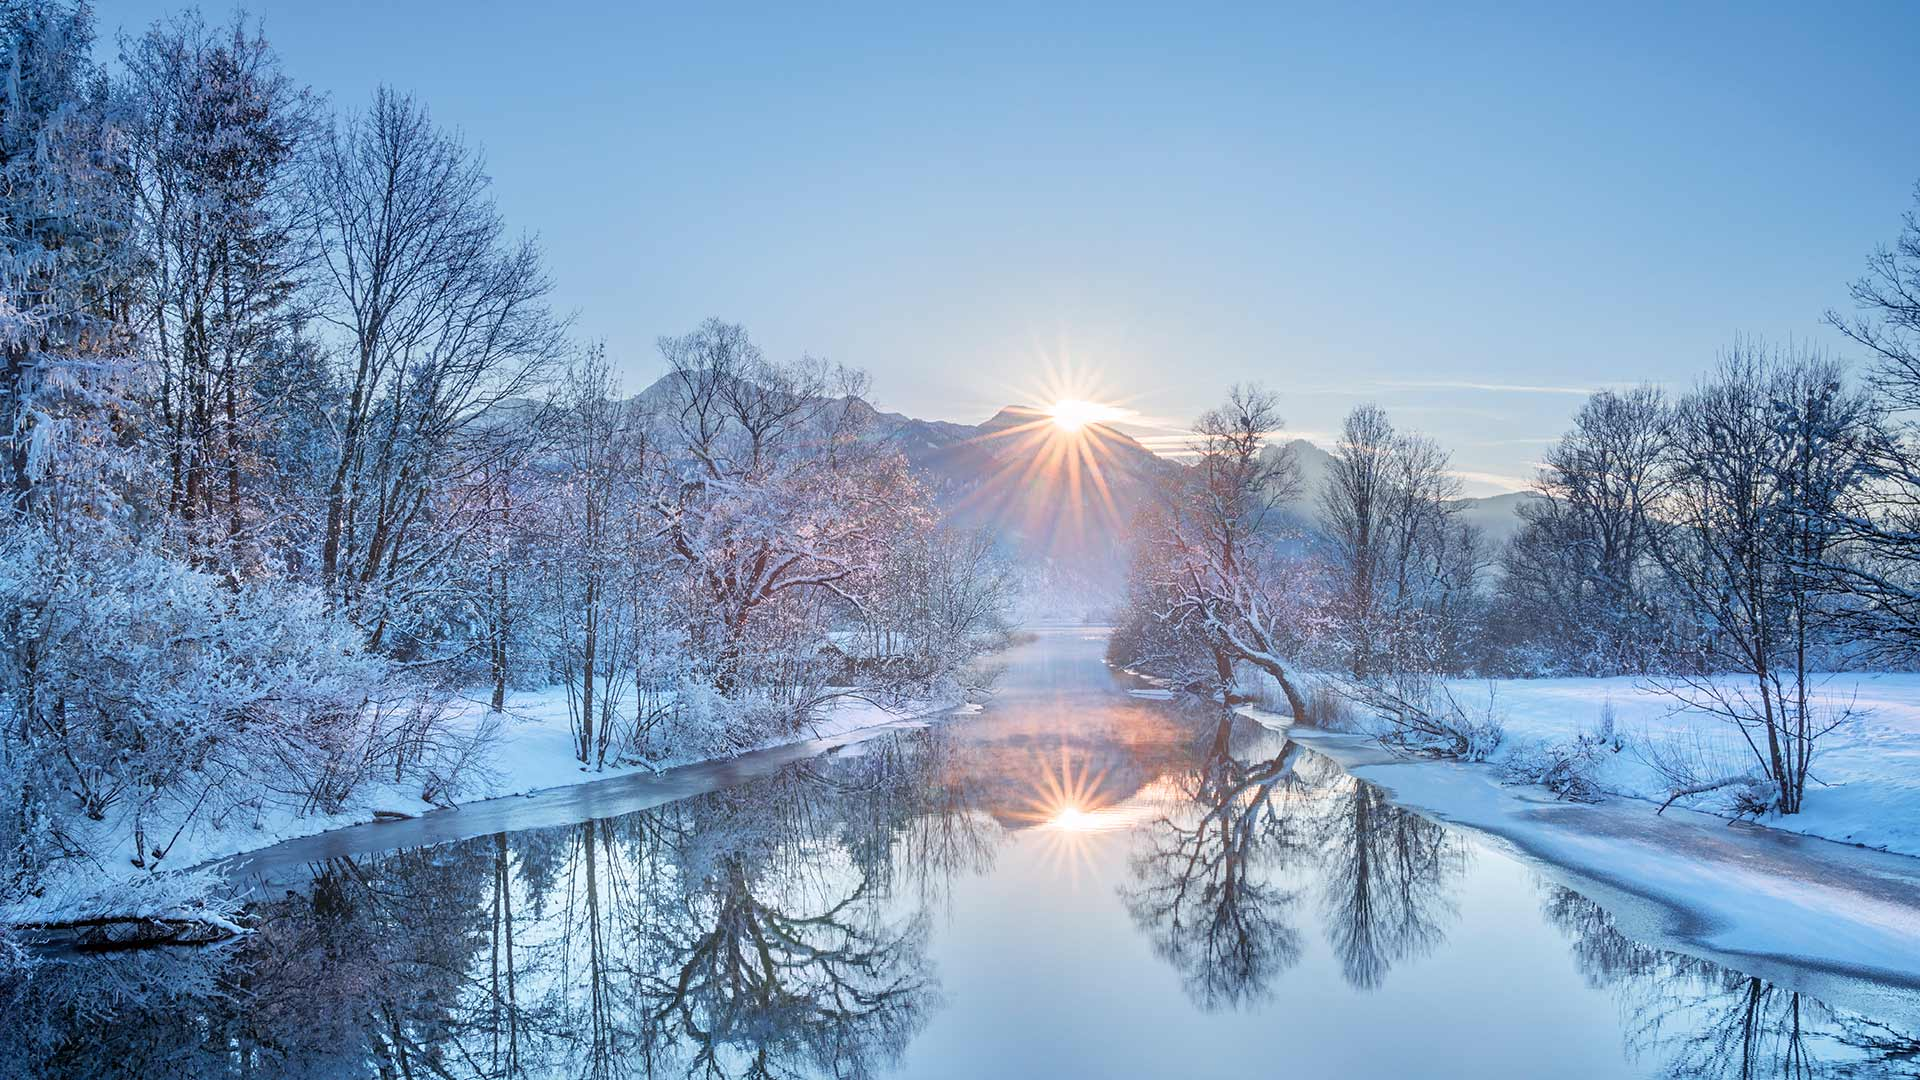
\includegraphics[width = .9\textwidth]{a.jpg}
\caption{有图有真相}
\label{fig:myphoto}
\end{figure}








\end{document}